\section{Results}

Given sets $D$ and $E$ such that
$f : D \rightarrow E$ for $f$ a Boolean function,
we construct matrices corresponding to the constraints
in \cref{Eq:boyd_obj}.
Our implementation uses Python3 and the NumPy library:
We build $A_i$ for $i \in [|F|]$ to enforce the condition
outlined in \cref{Eq:off-diag} and set $b_i=1$.
We build $\Ap_i$ for $i \in [|D|]$ to enforce
that $z$ is the maximum $c_i$ and set $\bp_i = 0$.
Finally, we build $C$ to select $z$ from $\Xb$.

To solve the SDP with our constraints,
we implemented Wen et al.'s ADM algorithm.
We again use Python3 and the NumPy library
in our implementation.

\subsection{OR Function: All Boolean Inputs}

So far we have illustrated the SDP and its solution
through the example of the OR function.
Recall that OR takes as input $n$ bit strings
and returns 0 if there are no 1s in the input
and 1 otherwise.
We extend our analysis of OR by illustrating
an application of our SDP solver.

\begin{figure}[ht]
\centering
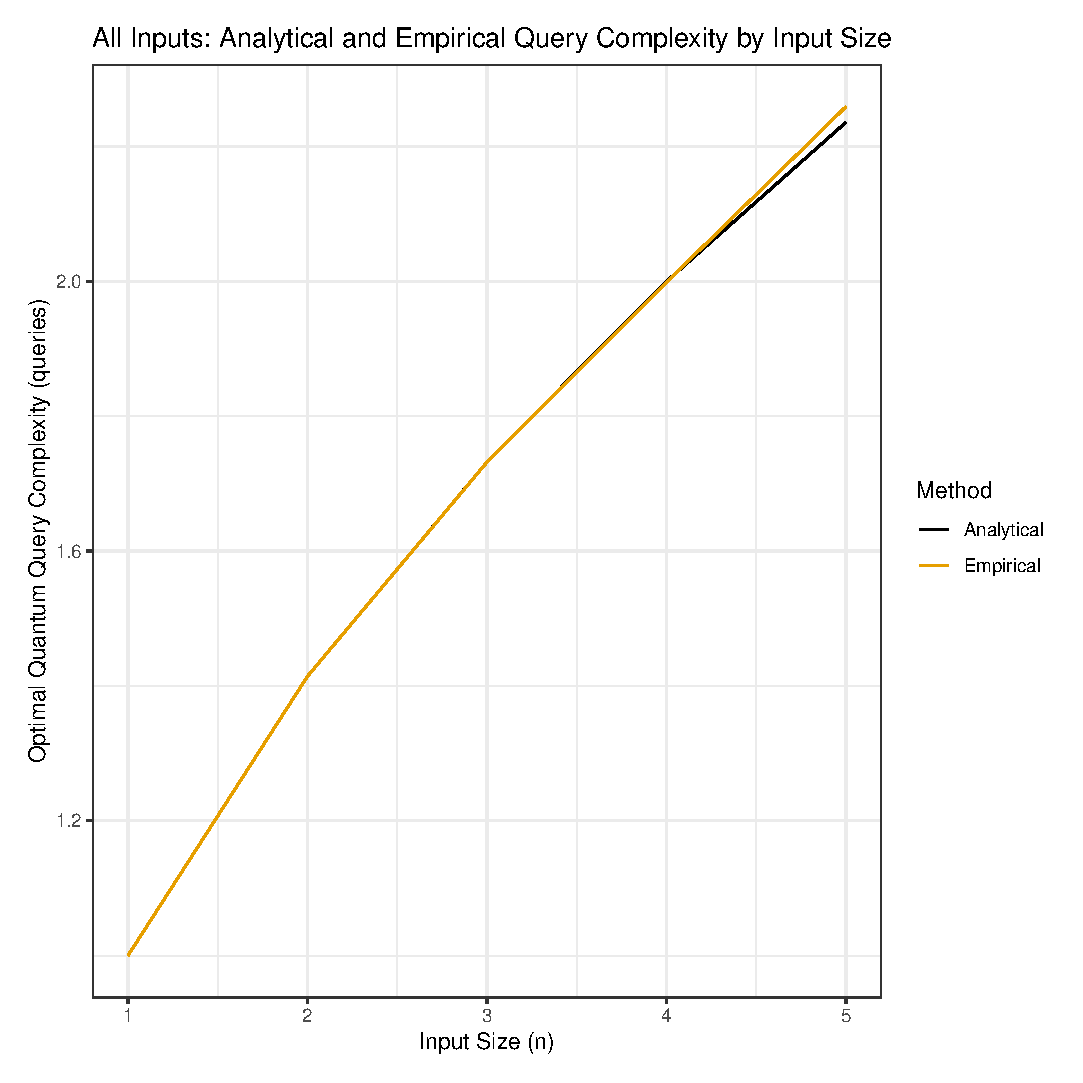
\includegraphics[scale=.3]{figure_all_or_complexity}
\caption{The }
\end{figure}

\subsection{OR Function: Worst-case Boolean Inputs}\label{sec:speed}

Limit to worst-case inputs to Boolean function

Quantum algorithm is very smart ;)

It does searches for worst-case as in \cref{Eq:off-diag}